\documentclass[12pt]{report}
\usepackage[utf8]{inputenc}
\usepackage[T1]{fontenc}
\usepackage[russian]{babel}
%\usepackage[14pt]{extsizes}
\usepackage{multirow}
\usepackage{listings}
\usepackage{graphicx}
\graphicspath{ {./img/} }
\usepackage{amsmath,amsfonts,amssymb,amsthm,mathtools} 
\usepackage{titlesec}
\usepackage{geometry}
\usepackage{caption}
\usepackage[hidelinks]{hyperref}
\usepackage{amsmath}

\frenchspacing
\usepackage{indentfirst} % Красная строка

\lstset{ %
basicstyle=\small\sffamily, % размер и начертание шрифта для подсветки кода
numbers=left,               % где поставить нумерацию строк (слева\справа)
numberstyle=\tiny,           % размер шрифта для номеров строк
stepnumber=1,                   % размер шага между двумя номерами строк
numbersep=5pt,                % как далеко отстоят номера строк от подсвечиваемого кода
showspaces=false,            % показывать или нет пробелы специальными отступами
showstringspaces=false,      % показывать или нет пробелы в строках
showtabs=false,             % показывать или нет табуляцию в строках
frame=single,              % рисовать рамку вокруг кода
tabsize=2,                 % размер табуляции по умолчанию равен 2 пробелам
captionpos=t,              % позиция заголовка вверху [t] или внизу [b] 
breaklines=true,           % автоматически переносить строки (да\нет)
breakatwhitespace=false, % переносить строки только если есть пробел
escapeinside={\#*}{*)}   % если нужно добавить комментарии в коде
}

\geometry{pdftex, left = 3cm, right = 10mm, top = 2cm, bottom = 2cm}

% Для измененных титулов глав:
\usepackage{titlesec, blindtext, color} % подключаем нужные пакеты
\definecolor{gray75}{gray}{0.75} % определяем цвет
\newcommand{\hsp}{\hspace{20pt}} % длина линии в 20pt

% caption for tables at top
\usepackage{float}
\floatstyle{plaintop}
\restylefloat{table}

\titleformat{\chapter}[hang]{\Huge\bfseries}{\thechapter\hsp\textcolor{gray75}{|}\hsp}{0pt}{\Huge\bfseries}

\title{Lab 01 report}
\author{Kirill}

\date{\today}

\begin{document}
\thispagestyle{empty}

\noindent \begin{minipage}{0.15\textwidth}
	
\includegraphics[width=\linewidth]{b_logo}
\end{minipage}
\noindent\begin{minipage}{0.85\textwidth}\centering
	\textbf{Министерство науки и высшего образования Российской Федерации}\\
	\textbf{Федеральное государственное бюджетное образовательное учреждение высшего образования}\\
	\textbf{«Московский государственный технический университет имени Н.Э.~Баумана}\\
	\textbf{(национальный исследовательский университет)»}\\
	\textbf{(МГТУ им. Н.Э.~Баумана)}
\end{minipage}

\noindent\rule{16cm}{3pt}
\newline\newline
\noindent ФАКУЛЬТЕТ $\underline{\text{«Информатика и системы управления»}}$ \newline\newline
\noindent КАФЕДРА $\underline{\text{«Программное обеспечение ЭВМ и информационные технологии»}}$\newline\newline\newline\newline\newline\newline\newline


\begin{center}
	\noindent\begin{minipage}{1.3\textwidth}\centering
	\Large\textbf{   ~~~ Лабораторная работа №1}\newline
	\textbf{по дисциплине "Анализ Алгоритмов"}\newline\newline\newline
	\end{minipage}
\end{center}

\noindent\textbf{Тема} $\underline{\text{Расстояние Левенштейна}}$\newline\newline
\noindent\textbf{Студент} $\underline{\text{Рядинский К. В.}}$\newline\newline
\noindent\textbf{Группа} $\underline{\text{ИУ7-53Б}}$\newline\newline
\noindent\textbf{Преподаватель} $\underline{\text{Волкова Л. Л.}}$\newline

\begin{center}
	\mbox{}
	\vfill
	Москва
\end{center}

\begin{center}
	\the\year ~г.
\end{center}
\clearpage


\tableofcontents
\newpage

\chapter*{Введение}
\addcontentsline{toc}{chapter}{Введение}
	
\textbf{Расстояние Левенштейна} - минимальное количество операций вставки одного символа, удаления одного символа и замены одного символа на другой, необходимых для превращения одной строки в другую.

Расстояние Левенштейна применяется в теории информации и компьютерной лингвистике для следущего:

\begin{itemize}
	\item исправления ошибок в слове;
	\item сравнения текстовых файлов утилитой diff;
	\item в биоинформатике для сравнения генов, хромосом и белков.
\end{itemize}

Цели данной лабораторной работы: 
\begin{enumerate}
	\item Изучение метода динамического программирования на материале алгоритмов нахождения расстояния Левенштейна и Дамерау-Левенштейна.
	\item Оценка реализаций алгоритмов нахождения расстояния Левенштейна и Дамерау-Левенштейна.
\end{enumerate}

Задачами данной лабораторной являются:
\begin{enumerate}
	\item Изучение алгоритмов Левенштейна и Дамерау-Левенштейна нахождения расстояния между строками;
	\item Применение метода динамического программирования для матричной реализации указанных алгоритмов; 
	\item Получение практических навыков реализации указанных алгоритмов: двух алгоритмов в матричной версии и одного из алгоритмов в рекурсивной версии; 
	\item Сравнительный анализ линейной и рекурсивной реализаций выбранного алгоритма определения расстояния между строками по затрачиваемым ресурсам (времени и памяти); 
	\item Экспериментальное подтверждение различий во временнóй эффективности рекурсивной и
	      нерекурсивной реализаций выбранного алгоритма определения расстояния между строками при
	      помощи разработанного программного обеспечения на материале замеров процессорного времени
	      выполнения реализации на варьирующихся длинах строк; 
	\item Описание и обоснование полученных результатов в отчете о выполненной лабораторной
	      работе, выполненного как расчётно-пояснительная записка к работе. 
\end{enumerate}

\chapter{Аналитическая часть}
Расстояние Левенштейна [2] между двумя строками ~--~ это минимальное количество операций вставки, удаления и замены, необходимых для превращения одной строки в другую

Цены операций могут зависеть от вида операций (вставка, удаление, замена) и/или от участвующих в ней символов, отражая разную вероятность разных ошибок при вводе текста и т.п. В общем случае

\begin{itemize}
	\item $w(a, b)$ ~--~ цена замены символа $a$ на $b$
	\item $w(\lambda, b)$ ~--~ цена вставки символа $b$
	\item $w(a, \lambda)$ ~--~ цена удаления символа $a$
\end{itemize}

Для решения задачи о редакционном расстоянии необходимо найти последовательность замен, минимизирующую суммарную цену. Расстояние Левенштейна является частным случаем это задачи при

\begin{itemize}
	\item $w(a, a) = 0$
	\item $w(a, b) = 1$, $a \neq b$
	\item $w(\lambda, b) = 1$
	\item $w(a, \lambda) = 1$ 
\end{itemize}

\section{Расстояние Левенштейна}

Пусть $S_{1}$ и $S_{2}$ — две строки (длиной M и N соответственно) над некоторым алфавитом, тогда расстояние Левенштейна можно подсчитать по следующей рекуррентной формуле:

\begin{displaymath}
	D(i,j) = \left\{ \begin{array}{ll}
	0, & \textrm{$i = 0, j = 0$}\\
	i, & \textrm{$j = 0, i > 0$}\\
	j, & \textrm{$i = 0, j > 0$}\\
	min(\\
	D(i,j-1)+1,\\
	D(i-1, j) +1, &\textrm{$j>0, i>0$}\\
	D(i-1, j-1) + m(S_{1}[i], S_{2}[j])\\
	),
	\end{array} \right.
\end{displaymath}

\noindent
где $m(a,b)$ равна нулю, если $a=b$ и единице в противном случае; $min\{\,a,b,c\}$ возвращает наименьший из аргументов.

\section{Расстояние Дамерау-Левенштейна}

Расстояние Дамерау-Левенштейна вычисляется по следующей рекуррентной формуле:
		    
\[ D(i, j) =  \left\{
	\begin{aligned}
		  & 0, &   & i = 0, j = 0 \\
		  & i, &   & i > 0, j = 0 \\
		  & j, &   & i = 0, j > 0 \\		    	
		&min \left\{
		\begin{aligned}
		&D(i, j - 1) + 1,\\
		&D(i - 1, j) + 1,\\
		&D(i - 1, j - 1) + m(S_{1}[i], S_{2}[i]), \\
		&D(i - 2, j - 2) + m(S_{1}[i], S_{2}[i]),\\
	\end{aligned} \right.
	&& 
	\begin{aligned}
		  & , \text{ если } i, j > 0         \\
		  & \text{ и } S_{1}[i] = S_{2}[j - 1]  \\
		  & \text{ и } S_{1}[i - 1] =  S_{2}[j] \\
	\end{aligned} \\ 
	&min \left\{
	\begin{aligned}
		  & D(i, j - 1) + 1,                         \\
		  & D(i - 1, j) + 1,                         \\
		  & D(i - 1, j - 1) + m(S_{1}[i], S_{2}[i]), \\
	\end{aligned} \right.  &&, \text{иначе}
	\end{aligned} \right.
\]	
	    
\section{Вывод}
В данном разделе были рассмотрены алгоритмы нахождения расстояния Левенштейна и Дамерау-Левенштейна, который является модификаций первого, учитывающего возможность перестановки соседних символов. 
		
\chapter{Конструкторская часть}
На рис. \ref{fig:rec_lev} приведена схема рекурсивного алгоритма Левенштейна

На рис. \ref{fig:rec_dam_lev} приведена схема рекурсивного алгоритма Дамерау-Левенштейна

На рис. \ref{fig:iter_lev} приведена схема матричного алгоритма Левенштейна

На рис. \ref{fig:iter_dam_lev} приведена схема матричного алгоритма Дамерау-Левенштейна

\section{Схемы алгоритмов}

\begin{figure}[h]
	\centering
	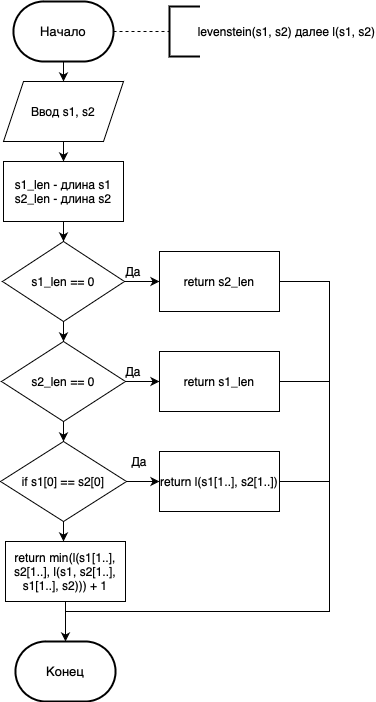
\includegraphics[scale=0.9]{lev_rec.png}
	\caption{Схема рекурсивного алгоритма нахождения расстояния Левенштейна}
	\label{fig:rec_lev}
\end{figure}

\begin{figure}[h]
	\centering
	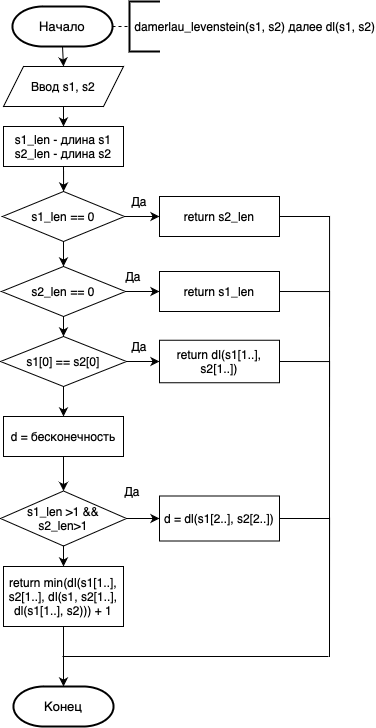
\includegraphics[scale=0.85]{dam_lev_rec.png}
	\caption{Схема рекурсивного алгоритма нахождения расстояния Дамерау-Левенштейна}
	\label{fig:rec_dam_lev}
\end{figure}

\begin{figure}[h]
	\centering
	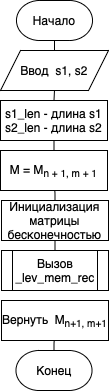
\includegraphics[scale=1]{lev_cache_main.png}
	\caption{Схема рекурсивного алгоритма нахождения расстояния Левенштейна с кэшем}
	\label{fig:rec_lev_cache_main}
\end{figure}

\begin{figure}[h]
	\centering
	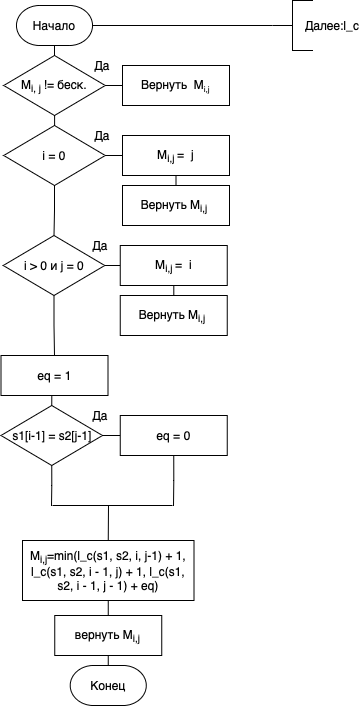
\includegraphics[scale=0.85]{lev_cache_aux.png}
	\caption{Схема подпрограммы алгоритмы нахождения расстояния Левенштейна с кэшем}
	\label{fig:rec_lev_cache_aux}
\end{figure}

\begin{figure}[h]
	\centering
	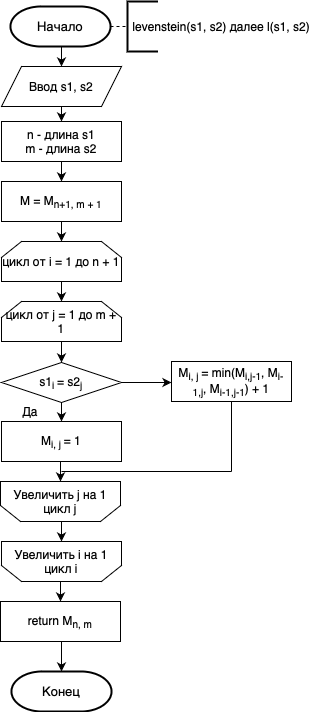
\includegraphics[scale=0.9]{lev_iter.png}
	\caption{Схема матричного алгоритма нахождения расстояния Левенштейна}
	\label{fig:iter_lev}
\end{figure}

\begin{figure}[h]
	\centering
	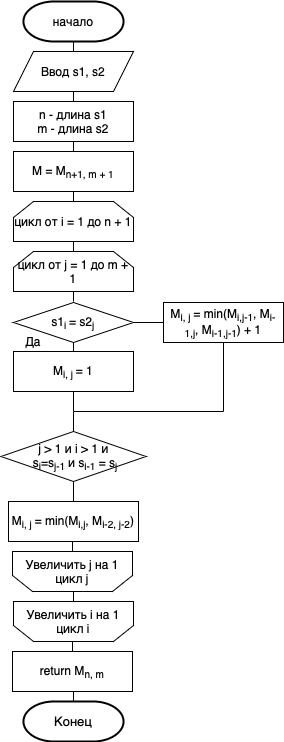
\includegraphics[width=0.5\linewidth]{dam_lev_iter.png}
	\caption{Схема матричного алгоритма нахождения расстояния Дамерау-Левенштейна}
	\label{fig:iter_dam_lev}
\end{figure}

\chapter{Технологическая часть}

В данном разделе приведены требования к программному обеспечению (далее ~--~ ПО), средства реализации и листинги кода

\section{Требования к ПО}

\textbf{Требования к вводу}
		
\begin{enumerate}
	\item На вход подаются две строки
	\item Заглавные и прописные буквы считаются разными
\end{enumerate}
		
\textbf{Требования к программе:}

\begin{enumerate}
	\item Две пустые строки - корректный ввод, программа не должна аварийно завершаться
\end{enumerate}

\clearpage


\section{Выбор языка программирования}
Для реализации программ я выбрал язык программирования Rust [1], так как этот язык предоставляет как низкоуровневые интерфейсы, так и высокоуровневые. Также он является таким же быстрым, как и С++, но более безопасен. Среда разработки Visual Studio Code.

\section{Листинги реализации алгоритма}

В данных рекурсивных реализациях в связи с особенностями языка Rust, индексация строк идет от нуля и на каждый рекурсивный вызов в функцию передается подстрока от 1 элемента до n.
\begin{equation*} 
	String = \{ c_1, c_2, \dotso c_n \}
\end{equation*}

\begin{equation*}
	Substring = \{ c_2, \dotso c_n \},  Substring \in String, n \in \mathbb{N}
\end{equation*}
		
\begin{lstlisting}[label=some-code,caption=Функция нахождения расстояния Левенштейна рекурсивно]
pub fn levenstein_rec(s1: &str, s2: &str) -> usize {
	let s1_len = s1.len();
	let s2_len = s2.len();

	if s1_len == 0 {
		return s2_len;
	}

	if s2_len == 0 {
		return s1_len;
	}   

	if s1.chars().nth(0) == s2.chars().nth(0) {
		return levenstein_rec(&s1[1..], &s2[1..]);
	}

	let a = levenstein_rec(&s1[1..], &s2[1..]);
	let b = levenstein_rec(s1, &s2[1..]);
	let c = levenstein_rec(&s1[1..], &s2);

	return std::cmp::min(a, std::cmp::min(b, c)) + 1;
}
\end{lstlisting}

\newpage

\begin{lstlisting}[label=some-code,caption=Функция нахождения расстояния Дамерау-Левенштейна рекурсивно]
pub fn damerau_levenstein_rec(s1: &str, s2: &str) -> usize {
	let s1_len = s1.len();
	let s2_len = s2.len();

	if s1_len == 0 {
		return s2_len;
	}

	if s2_len == 0 {
		return s1_len;
	}   

	if s1.chars().nth(0) == s2.chars().nth(0) {
		return damerau_levenstein_rec(&s1[1..], &s2[1..]);
	}

	let a = damerau_levenstein_rec(&s1[1..], &s2[1..]);
	let b = damerau_levenstein_rec(s1, &s2[1..]);
	let c = damerau_levenstein_rec(&s1[1..], &s2);

	let mut d = usize::MAX;
	if s1_len > 1 && s2_len > 1 {
		d = damerau_levenstein_rec(&s1[2..], &s2[2..]);
	}

	return std::cmp::min(d, std::cmp::min(a, std::cmp::min(b, c))) + 1;
}

\end{lstlisting}

\clearpage

\begin{lstlisting}[label=some-code,caption=Функция нахождения расстояния Левенштейна рекурсивно с кэшем]
fn _levenstein_mem_rec(s1: &Vec<char>, s2: &Vec<char>, i: usize, j: usize, matrix: & mut Vec<Vec<usize>>) -> usize {
    if matrix[i][j] != usize::MAX {
        return matrix[i][j];
    }

    if i == 0 {
        matrix[i][j] = j;
        return matrix[i][j];
    }

    if j == 0 && i > 0 {
        matrix[i][j] = i;
        return matrix[i][j];
    }

    let mut eq = 1;

    if s1[i - 1] == s2[j - 1] {
        eq = 0;
    }

    matrix[i][j] = std::cmp::min(
        _levenstein_mem_rec(s1, s2, i, j - 1, matrix) + 1,
        std::cmp::min(
            _levenstein_mem_rec(s1, s2, i - 1, j, matrix) + 1,
            _levenstein_mem_rec(s1, s2, i - 1, j - 1, matrix) + eq
        )
    );

    return matrix[i][j];
}

pub fn levenstein_mem_rec(s1: &str, s2: &str) -> usize {
    let w1 = s1.chars().collect::<Vec<_>>();
    let w2 = s2.chars().collect::<Vec<_>>();

    let word1_length = w1.len();
    let word2_length = w2.len();

    let mut matrix = vec![vec![0; word1_length + 1]; word2_length + 1];

    for i in 0..word1_length + 1 {
        for j in 0..word2_length + 1 {
            matrix[i][j] = usize::MAX;
        }
    }

    _levenstein_mem_rec(&w1, &w2, word1_length, word2_length, &mut matrix);

    return matrix[word1_length][word2_length];
}
\end{lstlisting}

\newpage

\begin{lstlisting}[label=some-code,caption=Функция нахождения расстояния Левенштейна матрично]
pub fn levenstein_iter(word1: &str, word2: &str) -> usize {
	// getting length of words
	let w1 = word1.chars().collect::<Vec<_>>();
	let w2 = word2.chars().collect::<Vec<_>>();

	let word1_length = w1.len() + 1;
	let word2_length = w2.len() + 1;

	let mut matrix = vec![vec![0; word1_length]; word2_length];

	for i in 1..word1_length {
		matrix[0][i] = i;
	}
	for j in 1..word2_length {
		matrix[j][0] = j;
	}

	for j in 1..word2_length {
		for i in 1..word1_length {
			let x: usize = if w1[i - 1] == w2[j - 1] {
				matrix[j - 1][i - 1]
			} else {
				1 + std::cmp::min(
					std::cmp::min(matrix[j][i - 1], matrix[j - 1][i]),
					matrix[j - 1][i - 1],
				)
			};
			matrix[j][i] = x;
		}
	}
	return matrix[word2_length - 1][word1_length - 1];
}
\end{lstlisting}

\newpage

\begin{lstlisting}[label=some-code,caption=Функция нахождения расстояния Дамерау-Левенштейна матрично]
pub fn damerau_levenstein_iter(word1: &str, word2: &str) -> usize {
    // getting length of words
    let w1 = word1.chars().collect::<Vec<_>>();
    let w2 = word2.chars().collect::<Vec<_>>();

    let word1_length = w1.len() + 1;
    let word2_length = w2.len() + 1;

    let mut matrix = vec![vec![0; word1_length]; word2_length];

    for i in 1..word1_length {
        matrix[0][i] = i;
    }
    for j in 1..word2_length {
        matrix[j][0] = j;
    }

    for j in 1..word2_length {
        for i in 1..word1_length {
            let x: usize = if w1[i - 1] == w2[j - 1] {
                matrix[j - 1][i - 1]
            } else {
                1 + std::cmp::min(
                    std::cmp::min(matrix[j][i - 1], matrix[j - 1][i]),
                    matrix[j - 1][i - 1],
                )
            };

            matrix[j][i] = x;

            if (j > 1) && (i > 1) && (w1[i - 1] == w2[j - 2]) && (w1[i - 2] == w2[j - 1]) {
                matrix[j][i] = std::cmp::min(x, matrix[j - 2][i - 2] + 1);
            }
        }
    }
    return matrix[word2_length - 1][word1_length - 1];
}
\end{lstlisting}

\clearpage

В Таблице \ref{tab:func_tests} приведены функциональные тесты для алгоритмов вычисления расстояния Левенштейна и Дамерау-Левенштейна.

Все тесты были пройдены успешно (ожидаемый результат совпал с фактическим).

\begin{table}[h]
	\centering
	\begin{tabular}{|c|c|c|c|}
		\hline
		\multirow{2}{*}{Строка 1} & \multirow{2}{*}{Строка 2} & \multicolumn{2}{c|}{Ожидаемый результат} \\ \cline{3-4} 
		&          & Левенштейн & Дамерау-Левенштейн \\ \hline
		Take   & Took     & 3          & 3                   \\ \hline
		Art    & Atr      & 2          & 1                   \\ \hline
		car    & city     & 3          & 3                   \\ \hline
		head   & ehda     & 3          & 2                   \\ \hline
		laptop & notebook & 7          & 7                   \\ \hline
		peek   & peeks    & 1          & 1                   \\ \hline
		rain   & pain     & 1          & 1                   \\ \hline
	\end{tabular}
	\caption{Функциональные тесты}
	\label{tab:func_tests}
\end{table}
	
	\chapter{Исследовательская часть}
	В данном разделе будут представлены замеры времени работы реализаций алгоритмов и потребления памяти
	
	\section{Сравнительный анализ на основе замеров времени работы алгоритмов}
	
	Был проведен замер времени работы каждого из алгоритмов с помощью библиотеки Criterion [3]. Эта библиотека замеряет процессорное время выполнения функции и усредняет его. В таблице \ref{tab:bench} содержится результат исследований.

	Замер времени был выполнен со строками одинаковой длины. Длина строки ~--~ количество символов, содержащихся в этой строке.
	
	\begin{table}[h]
		\centering
		\begin{tabular}{|c|c|c|c|c|c|}
		\hline
		\multicolumn{1}{|l|}{Длина слов} &
		  \multicolumn{1}{l|}{Лев рек.} &
		  \multicolumn{1}{l|}{Лев итер.} &
		  \multicolumn{1}{l|}{Лев. рек. кэш} &
		  \multicolumn{1}{l|}{Дам-Лев рек.} &
		  \multicolumn{1}{l|}{Дам-Лев итер.} \\ \hline
		1 & 8,50E-08 & 2,48E-07 & 2,58E-07 & 3,20E-10 & 5,50E-07 \\ \hline
		2 & 1,08E-07 & 3,07E-07 & 3,63E-07 & 4,80E-08 & 4,93E-07 \\ \hline
		3 & 3,20E-07 & 4,26E-07 & 4,95E-07 & 2,77E-07 & 4,91E-07 \\ \hline
		4 & 1,30E-06 & 4,88E-07 & 6,46E-07 & 1,50E-06 & 5,00E-07 \\ \hline
		5 & 6,90E-06 & 7,41E-07 & 9,02E-07 & 8,40E-06 & 5,08E-07 \\ \hline
		6 & 3,65E-05 & 8,12E-07 & 1,00E-06 & 4,68E-05 & 5,31E-07 \\ \hline
		7 & 1,97E-04 & 9,86E-07 & 1,26E-06 & 2,64E-04 & 5,14E-07 \\ \hline
		8 & 1,00E-03 & 1,10E-06 & 1,47E-06 & 1,51E-03 & 5,20E-07 \\ \hline
		9 & 5,92E-03 & 1,22E-06 & 1,71E-06 & 8,72E-03 & 5,09E-07 \\ \hline
		\end{tabular}
		\caption{Время работы алгоритмов (в секундах)}
		\label{tab:bench}
		\end{table}

	\pagebreak

	На рис. \ref{fig:plot} представлена зависимость времени работы реализаций алгоритмов от длины строк. Для удобства ось времени работы представлена в логарифмической шкале
	
	
	\begin{figure}[ht]
		\centering
		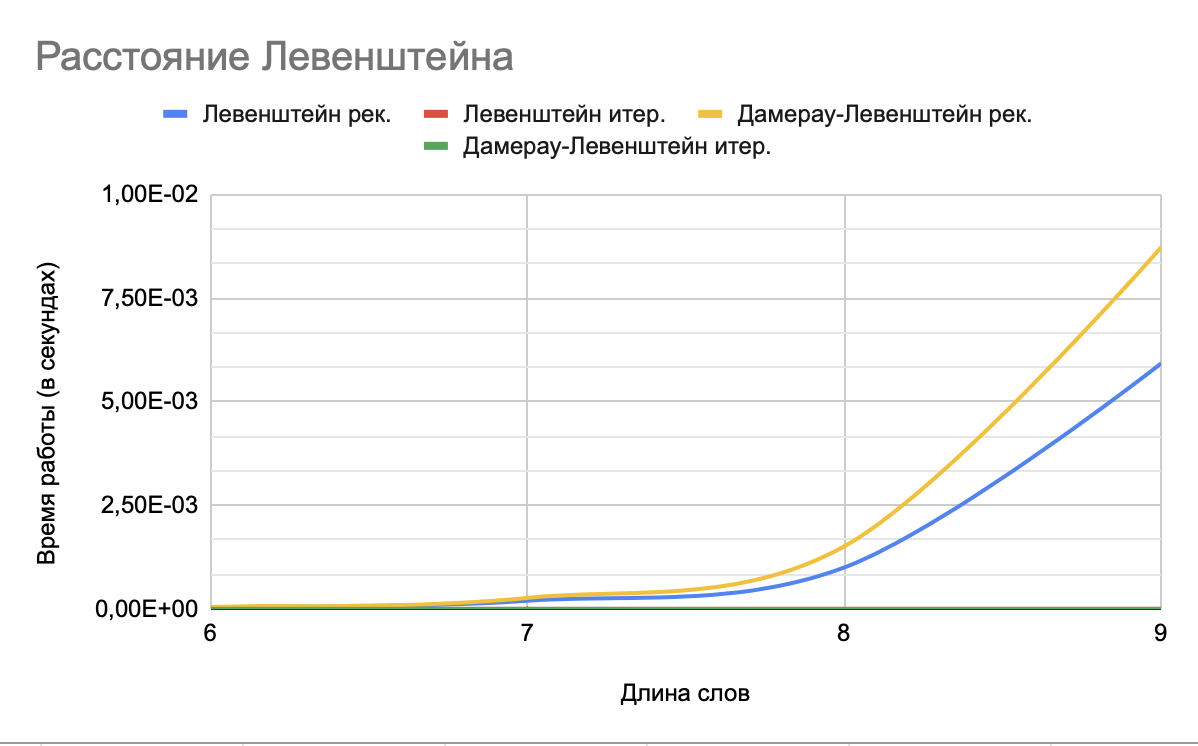
\includegraphics[width=0.75\textwidth]{plot.png}
		\caption{Зависимость времени работы алгоритмов от длины строк}
		\label{fig:plot}
	\end{figure}

	Наиболее эффективными по времени при маленькой длине слова являются рекурсивные реализации алгоритмов, но как только увеличивается длина слова, их эффективность резко снижается, что обусловлено большим количеством повторных рассчетов. Время работы алгоритма, использующего матрицу, намного меньше благодаря тому, что в нем требуется только (m + 1)*(n + 1) операций заполнения ячейки матрицы. Также установлено, что алгоритм Дамерау-Левенштейна работает немного дольше алгоритма Левенштейна, т.к. в нем добавлены дополнительные проверки, однако алгоритмы сравнимы по временной эффективности.

	\section{Использование памяти}

	\par
	Алгоритмы Левенштейна и Дамерау-Левенштейна не отличаются по использованию памяти, соответственно достаточно рассмотреть рекурсивный и матричный реализации этих алгоритмов.

	\par
	Максимальная глубина стека вызовов при рекурсивной реализации равна сумме длин входящих строк, а на каждый вызов функции требуется еще 5 дополнительных переменных типа \textit{usize}, соответственно, максимальный расход памяти

	\begin{equation}
		(Size(S_{1}) + Size(S_{2}) \cdot (2 \cdot Size(\text{string}) + 5 \cdot Size(\text{usize})))
	\end{equation}
	
	\noindent
	где Size - функция, возвращающая размер аргумента; string - строковый тип, usize - целочисленный, беззнаковый тип.

	\par
	Использование памяти при итеративной реализации теоритически равно

	\begin{equation}
		(Size(S_{1} + 1) \cdot Size(S_{2} + 1)) \cdot Size(usize) + 2 \cdot Size(string)
	\end{equation}

	\par
	Использование памяти рекурсивной реализации алгоритма Левенштейна с кэшем теоритически равно

	\begin{equation}
		(Size(S_{1}) + Size(S_{2}) \cdot (2 \cdot Size(\text{string}) + 5 \cdot Size(\text{usize})) + (Size(S_{1} + 1) \cdot Size(S_{2} + 1)) \cdot Size(usize) )
	\end{equation}

	\par
	В данный момент отсутствуют инструменты для замера потребления памяти для языка Rust, поэтому подробные и конкретные замеры невозможны.

	\section{Вывод}

	\par
	Рекурсивный алгоритм Левенштейна работает на порядок дольше итеративных реализаций, время его работы увеличивается в геометрической прогрессии. На словах длиной 9 символов, матричная реализация превосходит рекурсивную в 4800 раз. Рекурсивные алгоритмы Левенштейна и Дамерау - Левенштейна сопостовимы по времени. Однако, использование кэша значительно ускоряет рекурсивный алгоритм, но он все еще не превосходит матричную реализацию.

	\chapter*{Заключение}

	Был изучен метод динамического программирования на материале алгоритмов Левенштейна и Дамерау-Лев.
	Также изучены алгоритмы Левенштейна и Дамерау-Левенштейна нахождения расстояния между строками, получены практические навыки раелизации указанных алгоритмов
	в матричной  и рекурсивных версиях. 

	Экспериментально было подтверждено различие во временной эффективности рекурсивной и нерекурсивной реализаций выбранного алгоритма определения расстояния между строками при помощи разработаного программного обеспечения на материале замеров процессорного времени выполнения реализации на варьирующихся длинах строк. 

	В результате исследований можно сделать вывод, что матричная реализация данных алгоритмов заметно выигрывает по времени при росте длины строк, следовательно более применима в реальных проектах.
	
	При выполнение данной лабораторной работы были выполнены все цели и следующие задачи:

	\begin{itemize}
		\item Были изучены алгоритмов Левенштейна и Дамерау-Левенштейна нахождения расстояния между строками;
		\item Были применены методы динамического программирования для матричной реализации указанных алгоритмов;
		\item Были получены практические навыки реализации указанных алгоритмов: двух алгоритмов в матричной версии и одного из алгоритмов в рекурсивной версии;
		\item Были проведен сравнительный анализ линейной и рекурсивной реализаций выбранного алгоритма определения расстояния между строками по затрачиваемым ресурсам (времени и памяти);
		\item Было Экспериментально подтверждено различие во временнoй эффективности рекурсивной и нерекурсивной реализаций выбранного алгоритма определения расстояния между строками при помощи разработанного программного обеспечения на материале замеров процессорного времени выполнения реализации на варьирующихся длинах строк;
		\item Были описаны и обоснованы полученные результаты в отчете о выполненной лабораторной работе, выполненного как расчётно-пояснительная записка к работе.
	\end{itemize}

	\chapter*{Литература}

	\begin{enumerate}
		\item Блэнди Дж., Орендорф Дж. Программирование на языке Rust = Programming Rust. — ДМК Пресс, 2018. — 550 с. — ISBN 978-5-97060-236-2.
		\item В. И. Левенштейн. Двоичные коды с исправлением выпадений, вставок и замещений символов. Доклады Академий Наук СССР, 1965. 163.4:845-848.
		\item Criterion.rs - Statistics-driven benchmarking library for Rust [Электронный ресурс] \url{https://github.com/bheisler/criterion.rs} (дата обращения: \today)
	\end{enumerate}

\end{document}
